\section{基本RIP协议} % (fold)
\label{sec:rip}
	\subsection{协议概述} % (fold)
	\label{sub:协议概述}
		本项目中实现的RIP协议采用了RIPv1和RIPv2的协议规定的一部分,是一个基于DV算法的网络层路由协议。其主要算法是Bellman-Ford算法,路由费用以路由跳数作为度量,运行该协议的每个路由器能够计算出到其余路由器的下一跳路由以及路由费用。定义了请求报文和响应报文两种报文格式。为了尽可能避免环路和无穷计数问题,使用的机制包括毒性逆转(split-horizon with poison inverse)、延时刷新(flush timer)、触发更新(triggered update)、抑制更新(holddown)。在协议的扩展中,实现了该协议下适用的traceRoute功能。
	% subsection 协议概述 (end)
	\subsection{算法} % (fold)
	\label{sub:算法}
		\subsubsection{距离矢量表更新}
		\label{ssub:距离矢量表更新}
			距离矢量表计算主要基于Bellman-Ford算法。在基本的DV算法中,路由器每次收到邻居发来的距离矢量时,会使用Bellman-Ford的更新公式更新自己的距离矢量表:$$ dist_{self}(dest) = \min_{neighbour}\{dist_{neighbour}(dest) + metric(self,neighbour)\} $$ 为此,路由器需要在维护自己距离矢量表的同时,保存邻居发来的距离矢量表。
			\par 在RIP协议中,路由器只需保存和维护自己的距离矢量表。在收到邻居发来的距离矢量时,会将其与自己当前的距离矢量表进行比较,而不是用所有邻居的距离矢量表重新计算和比较。具体而言,RIP协议使用的更新公式为(假设收到邻居$nb$的距离矢量):$$ dist_{self}(dest) = \begin{cases} \min( dist_{self}(dest), dist_{nb}(dest) + metric(self,nb) ) & , nextHop_{self}(dest) \neq nb \\ dist_{nb}(dest) + metric(self,nb) & , nextHop_{self}(dest) = nb \end{cases}$$ 采用这种更新方式避免了路由器存储邻居距离矢量表的开销,也减少了更新所需的计算量。不足之处在于最短路径费用增加时,不能马上从其余路径中找到更优的并将其替代,需要等待其他邻居发送距离矢量。(事实上,为了避免环路和无穷计数问题,原最短路径费用增加后从其余路径中找替代的更新方式是不被允许的。)
		\subsubsection{环路与无限计数避免机制}
		\label{ssub:环路与无限计数避免机制}
			在本项目的实现中,为了尽可能避免环路与无限计数问题,使用了以下4种机制:
			\begin{itemize}
				\item 毒性逆转:一个路由器向邻居发的距离矢量中,下一跳为该邻居的项费用改为无穷(16)。
				\item 延迟刷新:一个路由器在与一个邻居失去连接(链路中断)后,不立即将其从距离矢量表中清除,而是延迟一段时间。在这段时间里,链路中断的信息能够告知其他路由。
				\item 触发更新:一个路由器在距离矢量表更新后,将更新的项立即向所有邻居发送。特别地,当一条链路断开后,触发更新会沿着包含这一链路的所有最短路径传播,从而使这些路径被毒化(即在路由器的转发表中费用为无穷)。
				\item 抑制更新:一个路由器在其一条最短路径被毒化后的一段时间内,忽略收到的一切声称能到达该路径目的地的距离矢量。这是为了避免在网络不稳定时使用邻居过时的路由信息进行更新。
			\end{itemize}
	% subsection 算法 (end)
	\subsection{协议特性} % (fold)
	\label{sub:协议特性}
	\subsubsection{协议流程} % (fold)
		\label{ssub:协议流程}
		本项目中实现的RIP协议主要包含的流程如下:
		\begin{enumerate}
			\item 路由器在进入区域时,向所有邻居发送request报文,邻居则返回一个response报文,里面含有邻居的距离矢量表。
			\item 该路由器会定时地向所有的邻居发送response报文,即自己的距离矢量表。
			\item 收到一个response报文意味着要维持该邻居的状态;而如果在一段时间内没有收到某个邻居路由器的response报文,则认为与该路由器的链路中断。
			\item 当收到其它邻居路由器的距离矢量表时,根据该信息更新自己的距离矢量表;当自己的距离矢量更新时,向所有邻居发送自己新的距离矢量表(只发送更新的部分)。
		\end{enumerate}
		% subsubsection 协议流程 (end)
	% subsection 协议特性 (end)
	\subsection{报文格式} % (fold)
	\label{sub:报文格式}
	本实验中使用的普通报文普通数据报文、request报文、response报文、TraceRoute报文、Echo报文如下:
	\par 普通报文:
	\begin{table}[H]
		\centering
		\begin{tabular}{|c|}
			\hline
			Command \\
			\hline
			source address \\
			\hline
			destination address \\
			\hline
			payload \\
			\hline
		\end{tabular}		
	\end{table}
	request报文:
	\begin{table}[H]
		\centering
		\begin{tabular}{|c|}
			\hline
			Command \; \vline \; Version \; \vline \; Routing domain \; \\
			\hline
			Source address \\
			\hline
			Address family \; \vline \; Route tag \; \\
			\hline
			address \\
			\hline
			Next hop \\
			\hline
			metric \\
			\hline
		\end{tabular}
	\end{table}
	Response报文:
	\begin{table}[H]
		\centering
		\begin{tabular}{|c|}
			\hline
			Command \; \vline \; Version \; \vline \; Routing domain \; \\
			\hline
			Source address \\
			\hline
			Address family \; \vline \; Route tag \; \\
			\hline
			address \\
			\hline
			Next hop \\
			\hline
			metric \\
			\hline
			repeat of last 17 bytes \\
			\hline
			$\cdots$ \\
			\hline 
		\end{tabular}	
	\end{table}
	TraceRoute报文:
	\begin{table}[H]
	\centering
		\begin{tabular}{|c|}
			\hline
			Command \\
			\hline
			source address \\
			\hline
			destination address \\
			\hline
			count \\
			\hline
		\end{tabular}		
	\end{table}	
	\newpage
	Echo 报文:
	\begin{table}[H]
	\centering
		\begin{tabular}{|c|}
			\hline
			Command \\
			\hline
			source address \\
			\hline
			destination address \\
			\hline
			local address \\
			\hline
		\end{tabular}		
	\end{table}
	报文项解释:
	\begin{enumerate}
		\item Command(1 Byte):指明这条报文的类型。
		\begin{enumerate}[]
			\item 0:普通报文。
			\item 1:请求报文。
			\item 2:响应(包含路由表)报文。
			\item 3:TraceRoute报文。
			\item 4:Echo报文。
		\end{enumerate}
		\item Version(1 Byte):RIP协议的版本。
		\item Routing domain(2 Bytes):指明这是RIP中的哪一步。
		\item Source address(6 Bytes):指明发送方的源地址和监听端口。
		\item Address family(2 Bytes):使用什么作为地址,使用IP该项为2。
		\item Route tag(2 Bytes):本项目中不用。
		\item address(6 Bytes):ip和端口号。
		\item Next hop(6 Bytes):下一跳路由的ip和端口。
		\item metric(1 Byte):代价度量(跳数)。
		\item Local address(6 Bytes):指明Echo报文发送者的源地址和监听端口。
		\item Count(1 Byte):路由跳数。
	\end{enumerate}
	% subsection 报文格式 (end)
	\subsection{协议扩展} % (fold)
	\label{sub:协议扩展}
		\begin{enumerate}
<<<<<<< HEAD
			\item 网络环路\\
				路由器可能收到自己发送的路由信息,因此造成网络环路。\\
				为了避免该情况,采用了:毒性逆转、抑制更新、触发更新和延迟刷新等机制。
			\item 无穷计数\\
				·采用延迟刷新,在检测到一个邻居可能失效时不立即将其从数据库中删除,等待一个间隔后再删除,目的是通告其它邻居该失效邻居不可达。
			\item TraceRoute\\
				·基于RIP路由16跳不可达这一机理,向目的地发跳数为1-16共16个报文,当一个路由器收到该报文,则提取其中的跳数,并将它减一。\\
				·当跳数为0时,向报文的源地址返回一个Echo报文;否则将跳数打包进原报文中,继续向目的地转发。\\
				·源地址路由器收集所有返回的Echo报文,如果5s内收到目的地址返回的Echo报文,则输出该路径;否则认为该目的地址不可达。
=======
			\item 处理网络环路和无穷计数
				\begin{itemize}
					\item 在网络状态变化时,路由器可能收到一条经过自身的的路径信息并以此更新距离矢量表,从而造成网络环路。通常情况下,网络环路会因为路径费用不断增加最终达到无穷而自动解决,但这极大影响了收敛速度。
					\item 为了尽可能避免环路,采用了毒性逆转、延迟刷新、抑制更新和触发更新等机制。
				\end{itemize}
			\item TraceRoute
				\begin{itemize}
					\item 基于RIP路由16跳不可达这一机理,向目的地发跳数为1-16共16个报文,当一个路由器收到该报文,则提取其中的跳数,并将它减一。
					\item 当跳数为0时,向报文的源地址返回一个Echo报文;否则将跳数打包进原报文中,继续向目的地转发。
					\item 源地址路由器收集所有返回的Echo报文,如果5s内收到目的地址返回的Echo报文,则输出该路径;否则认为该目的地址不可达。
				\end{itemize}
>>>>>>> 8cffb9f82ad63b95e64c115ae777d42918dd40d6
		\end{enumerate}
	% subsection 协议扩展 (end)
	\subsection{协议实现} % (fold)
	\label{sub:协议实现}
		本RIP协议基本由Python实现,主要利用的是socket库进行套接字编程并采用的是UDP协议、struct库进行数据的打包和解包、threading库管理线程和定时器。
		\par 实现方法实现了一个RIP协议类,处理内部流程和为外部调用留出了收发数据、查询路由路径等接口。
	% subsection 协议实现 (end)
	\subsection{结果} % (fold)
	\label{sub:结果}
		测试所用的拓扑图以及路由结果如下图\ref{fig:ripTest1}和\ref{fig:ripTest2}所示。
		\begin{figure}[H]
			\centering
			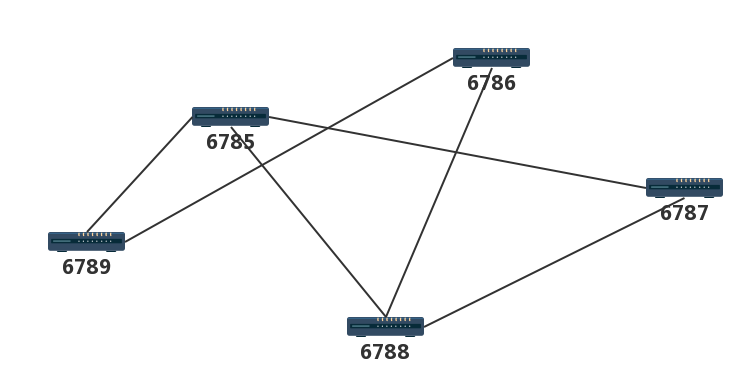
\includegraphics[scale=0.4]{imgs/topo1/tpop1.png}
			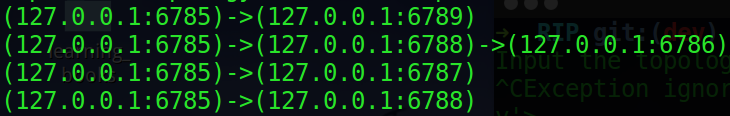
\includegraphics[scale=0.5]{imgs/ripTest1.PNG}
			\caption{RIP测试样例一}
			\label{fig:ripTest1}
		\end{figure}
		\begin{figure}[H]
			\centering
			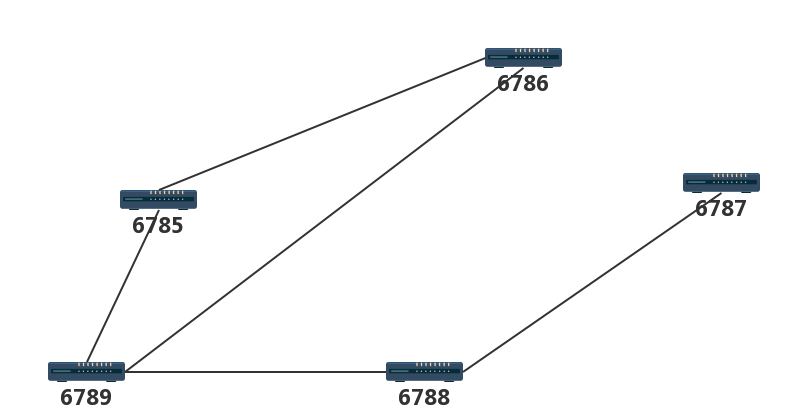
\includegraphics[scale=0.4]{imgs/topo1/topo2.png}
			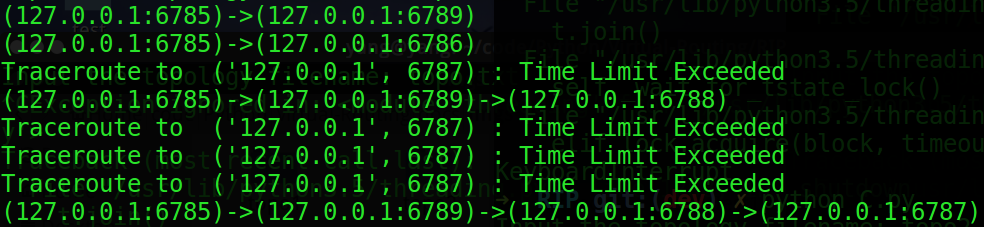
\includegraphics[scale=0.4]{imgs/ripTest2.PNG}
			\caption{RIP测试样例二}
			\label{fig:ripTest2}
		\end{figure}
		成功找出了其中的跳数最小的路径。
	% subsection 结果 (end)
	\subsection{总结} % (fold)
	\label{sub:总结}
		\begin{itemize}
			\item 原生的DV算法会因为RIP收敛速度缓慢,而产生路由环路的问题,而我们的RIP协议中采用了多种机制来解决了这种问题。
			\item 原生的DV算法需要保存邻居的路由表,而采用RIP协议的更新公式,避免了路由器存储邻居路由表的开销,而且减少了路由器更新时的计算量。
		\end{itemize}
	
	% subsection 总结 (end)


% section rip (end)